% Este archivo es parte de la memoria del proyecto fin de carrera
% de Manuel López Urbina. Protegida bajo la licencia GFDL.
% Para más información, la licencia completa viene incluida en el
% fichero fdl-1.3.tex

% Copyright (C) 2012 Manuel López Urbina

\chapter{Desarrollo software}
\label{chap:desarrollo-software}

\section{Metodología de desarrollo}

Este proyecto ha sido obtenido empleando una metodología de desarrollo basada en el modelo de construcción de prototipos para la parte software referente a la visión artificial y una metodología de desarrollo en cascada para el desarrollo de la interfaz gráfica y software de control del vehículo.\\

El modelo de construcción de prototipos proporciona una serie de características que lo hacen idóneo para este proyecto. Dicho modelo resulta especialmente útil en las siguientes situaciones:

\begin{itemize}
\item El cliente define los objetivos generales del software sin entrar en detalles pormenorizados de los requisitos de entrada, procesamiento o salida a obtener.
\item El responsable del desarrollo del software desconoce demasiados aspectos del desarrollo tales como, eficacia de un determinado algoritmo, capacidad de adaptación de un sistema operativo, definición de la interacción hombre-máquina entre otros.
\end{itemize}

Por otro lado, el modelo de desarrollo en cascada resulta adecuado para las siguientes situaciones:

\begin{itemize}
\item Se dispone de unos requisitos claros y precisos.
\item El sistema a desarrollar es de pequeña envergadura.
\item Las tecnologías utilizadas son conocidas por los desarrolladores.
\end{itemize}

Centrándonos nuevamente en el desarrollo del proyecto, los motivos que llevaron a cabo la elección del modelo de desarrollo por prototipos para la obtención del software de visión artificial fueron el amplio desconocimiento existente en cuanto a los algoritmos existentes y su eficacia e idoneidad al producto deseado. \\

En cambio, para el desarrollo de la interfaz gráfica y software de control del vehículo, se optó por el seguimiento del modelo de desarrollo en cascada al tratarse de un desarrollo con una menor dificultad técnica y la disponibilidad de los requisitos necesarios.\\

Por tanto el proyecto queda distribuido en tres subsistemas:

\begin{itemize}
\item Subsistema de visión artificial.
\item Subsistema de control.
\item Subsistema gráfico.
\end{itemize}


\begin{figure}[H]
  \begin{center}
    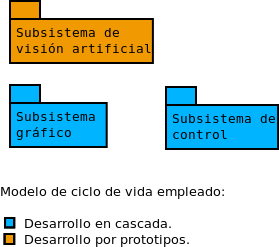
\includegraphics[scale=1]{subsistemas.png}
  \end{center}
  \caption{Subsistemas existentes en el proyecto junto con el modelo de ciclo de vida utilizado para su desarrollo.}
  \label{subsistemas}
\end{figure}

\section{Recolección de requisitos}

\subsection{Requisitos funcionales}

Para la elaboración de este proyecto se ha utilizado la metodología Métrica V3 así como el estándar ISO/IEC 12207. Métrica es una metodología de planificación, desarrollo y mantenimiento de los sistemas de información desarrollada por el Ministerio de Administraciones Públicas del Gobierno de España. Tiene como objetivo proporcionar una guía para la sistematización de actividades del ciclo de vida de los proyectos software en el ámbito de las administraciones públicas.\\

Métrica V3\cite{website:metrica} está basada en el modelo de procesos del ciclo de vida de desarrollo ISO/IEC 12207 (Information Technology - Software Life Cycle Processes) así como en la norma ISO/IEC 15504 SPICE (Software Process Improvement And Assurance Standards Capability Determination).\\

En la página oficial de Métrica V3, sus desarrolladores indican que puede ser utilizada libremente con la única restricción de citar la fuente de su propiedad intelectual, la del Ministerio de Administraciones Públicas.\\

Un caso de uso es una descripción de los pasos o actividades que deberán realizarse para llevar a cabo algún proceso. Los objetivos de los casos de uso son los siguientes:

\begin{itemize}
\item Obtener los requisitos funcionales del sistema y expresarlos desde un punto de vista más cercano al usuario.
\item Proporcionar una guía de todo el proceso de desarrollo del sistema de información. Los casos de uso proporcionan, por tanto, un modo claro y preciso de comunicación entre lo que desea el cliente y el desarrollador proporcionando desde el punto de vista del cliente una visión de ``caja negra'' del sistema eliminando los detalles de su construcción o desarrollo. Para los desarrolladores es utilizado como punto de partida y el eje sobre el que se apoya todo el desarrollo del sistema en los procesos de análisis y diseño.
\end{itemize}

Los requisitos funcionales que se han obtenido después del proceso de obtención de requisitos son los siguientes:

\begin{itemize}
\item Conectar con vehículo.
\item Desconectar con vehículo.
\item Pilotaje tradicional.
\item Pilotaje autónomo
\end{itemize}

\subsection{Diagramas de casos de uso}
\label{sec:casos-de-uso}

Los diagramas de caso de uso muestra una representación del comportamiento ofrecido por el sistema de información desde el punto de vista del usuario. El comportamiento del sistema es representado como un conjunto de transacciones ejecutadas entre el sistema y los actores junto con la descripción sobre las de las relaciones de comunicación existentes entre un actor y el sistema.\\

En la figura \ref{caso-de-uso} podemos observar el diagrama de casos de uso resultante tras la recolección de requisitos:\\

\begin{figure}[H]
  \begin{center}
    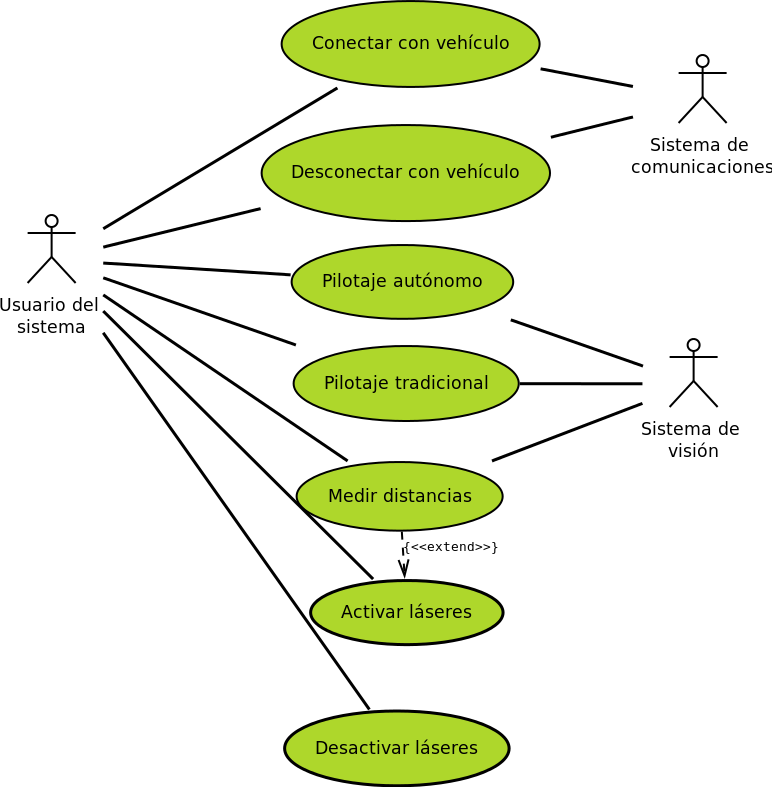
\includegraphics[scale=0.5]{diagrama-caso-de-uso.png}
  \end{center}
  \caption{Diagrama de casos de uso.}
  \label{caso-de-uso}
\end{figure}

\subsection{Especificación de los casos de uso}

A continuación se proporciona la especificaciones de cada uno de los casos de uso de la sección \ref{sec:casos-de-uso}.\\

\begin{table}[H]
  \begin{center}
    \begin{tabular}{|p{3.5cm}|p{10cm}|}
      \hline
      {\textbf{Caso de uso:}} & { Conexión coche.} \\
      \hline
      {\textbf{Descripción:}} & {El sistema deberá conectarse como describe el presente caso de uso cuando el operador del sistema desee conectar con el vehículo.} \\
     \hline
     \multicolumn{2}{c}{\emph{continua en la siguiente página ...}}\\
    \end{tabular}
  \end{center}
\end{table}    

\begin{table}[H]
  \begin{center}
    \begin{tabular}{|p{3.5cm}|p{10cm}|}
     \multicolumn{2}{c}{\emph{continua de la página anterior...}}\\
     \hline
      {\textbf{Actor principal:}} & { Operador del sistema.} \\
      \hline
      {\textbf{Actor secundario:}} & { Sistema de comunicaciones.} \\
     \hline
      {\textbf{Precondiciones:}} & { El sistema de comunicaciones deberá estar libre.} \\
     \hline     
     {\textbf{Flujo principal:}} & { 
\begin{enumerate}
\item El actor operador del sistema solicita establecer conexión con el coche.
\item El sistema comprueba que se puede establecer comunicación.
\item El sistema establece una conexión entre el ordenador personal y el coche mostrando por pantalla que la conexión se ha realizado exitosamente.
\end{enumerate}} \\
\hline
     {\textbf{Postcondición:}} & {Se establece una conexión entre el ordenador personal y el coche.}\\
     \hline
     {\textbf{Excepciones:}} & {Si no se encuentra el vehículo el sistema indicará error.}\\
     \hline
    \end{tabular}
  \end{center}
\caption{Descripción de caso de uso: Conexión coche.}
\end{table}


\begin{table}[H]
  \begin{center}
    \begin{tabular}{|p{3.5cm}|p{10cm}|}
      \hline
      {\textbf{Caso de uso:}} & { Desconexión del vehículo.} \\
      \hline
      {\textbf{Descripción:}} & { El sistema deberá actuar como describe en este caso de uso cuando el operador del sistema solicita la desconexión con el vehículo.} \\
     \hline
      {\textbf{Actor principal:}} & { Operador del sistema.} \\
      \hline
      {\textbf{Actor secundario:}} & { sistema de comunicaciones.} \\
      \hline
      {\textbf{Precondiciones:}} & { El sistema de comunicaciones deberá estar ocupado con una conexión activa.} \\
     \hline   
    {\textbf{Flujo principal:}} & { 
      \begin{enumerate}
\item El actor operador del sistema solicita la desconexión con el vehículo.
\item El sistema comprueba que se encuentra establecida una conexión entre el ordenador y el coche.
\item El sistema finaliza la conexión entre el ordenador y el vehículo e indica por pantalla que la desconexión se ha realizado con éxito.
\end{enumerate}
} \\
     \hline
     {\textbf{Postcondición}} & {Se finaliza la conexión entre el ordenador y el vehículo.}\\
     \hline
         {\textbf{Excepciones:}} & {No existe conexión entre el equipo y el vehículo.}\\
         \hline
    \end{tabular}
  \end{center}
\caption{Descripción del caso de uso: Desconexión coche.}
\end{table}

\begin{table}[H]
  \begin{center}
    \begin{tabular}{|p{3.5cm}|p{10cm}|}
      \hline
      {\textbf{Caso de uso:}} & { Pilotaje tradicional.} \\
      \hline
      {\textbf{Descripción:}} & {El sistema deberá comportarse como describe el presente caso de uso cuando el operador del sistema decida comenzar con el pilotaje tradicional del vehículo.} \\
     \hline
      {\textbf{Actor principal:}} & { Operador del sistema.} \\
      \hline
      {\textbf{Actor secundario:}} & {Sistema de visión artificial}\\
      \hline
      {\textbf{Precondiciones:}} & { Se encuentra establecida una conexión entre el ordenador y el vehículo y se están procesando imágenes.} \\
     \hline     
     {\textbf{Flujo principal:}} & { 
       \begin{enumerate}
       \item El actor operador del sistema solicita el pilotaje tradicional del vehículo.
       \item El sistema comprueba que existe una conexión activa entre el ordenador y el vehículo, y también que se están
         procesando imágenes.
       \item El sistema muestra las señales de tráfico detectadas en un momento determinado.
       \end{enumerate}
     } \\
     \hline
     {\textbf{Postcondición:}} & {Se comienza a pilotar el vehículo visualizándose las señales de tráfico del entorno.}\\
     \hline
     {\textbf{Excepciones:}} & {Si no se encuentra establecida la conexión entre el vehículo y el ordenador informa del error.}\\        
     \hline
    \end{tabular}
  \end{center}
\caption{Descripción del caso de uso: Pilotaje tradicional.}
\end{table}


\begin{table}[H]
  \begin{center}
    \begin{tabular}{|p{3.5cm}|p{10cm}|}
      \hline
      {\textbf{Caso de uso:}} & { Pilotaje autónomo.} \\
      \hline
      {\textbf{Descripción:}} & {El sistema deberá comportarse como describe el presente caso de uso cuando el operador del sistema decida comenzar con el pilotaje autónomo del vehículo.} \\
     \hline
      {\textbf{Actor principal:}} & { Operador del sistema.} \\
      \hline
      {\textbf{Actor secundario:}} & {Sistema de visión artificial}\\
      \hline
      {\textbf{Precondiciones:}} & { Se encuentra establecida una conexión entre el ordenador y el vehículo y se están procesando imágenes.} \\
     \hline 
    \multicolumn{2}{c}{\emph{continua en la siguiente página ...}}\\
    \end{tabular}
  \end{center}
\end{table}

\begin{table}[H]
  \begin{center}
    \begin{tabular}{|p{3.5cm}|p{10cm}|}
     \multicolumn{2}{c}{\emph{continua de la página anterior...}}\\
      \hline
     {\textbf{Flujo principal:}} & { 
       \begin{enumerate}
       \item El actor operador del sistema solicita el pilotaje autónomo del vehículo.
       \item El sistema comprueba que existe una conexión activa entre el ordenador y el vehículo, y también que se están
         procesando imágenes.
       \item El sistema muestra las señales de tráfico detectadas en un momento determinado.
       \item El vehículo realiza la operación correspondiente a la señal detectada.
       \end{enumerate}
     } \\
     \hline
     {\textbf{Postcondición:}} & {Se comienza a pilotar el vehículo visualizándose las señales de tráfico del entorno.}\\
     \hline
     {\textbf{Excepciones:}} & {Si no se encuentra establecida la conexión entre el vehículo y el ordenador informa del error.}\\        
     \hline
    \end{tabular}
  \end{center}
\caption{Descripción del caso de uso: Pilotaje autónomo.}
\end{table}


\begin{table}[H]
  \begin{center}
    \begin{tabular}{|p{3.5cm}|p{10cm}|}
      \hline
      {\textbf{Caso de uso:}} & { Medir distancias.} \\
      \hline
      {\textbf{Descripción:}} & {El sistema deberá mostrar la distancia a la que se encuentra un obstáculo del vehículo utilizando sus punteros láser.} \\
     \hline
      {\textbf{Actor principal:}} & { Operador del sistema.} \\
      \hline
      {\textbf{Actor secundario:}} & {Sistema de visión artificial}\\
      \hline
      {\textbf{Precondiciones:}} & { Se encuentra establecida una conexión entre el ordenador y el vehículo y se están procesando imágenes.} \\
     \hline 
     \multicolumn{2}{c}{\emph{continua en la siguiente página ...}}\\
    \end{tabular}
  \end{center}
\end{table}    

\begin{table}[H]
  \begin{center}
    \begin{tabular}{|p{3.5cm}|p{10cm}|}
     \multicolumn{2}{c}{\emph{continua de la página anterior...}}\\
     \hline
     {\textbf{Flujo principal:}} & { 
       \begin{enumerate}
       \item El actor operador del sistema solicita la medición de distancias.
       \item El sistema comprueba que existe una conexión activa entre el ordenador y el vehículo, y también que se están
         procesando imágenes.
       \item El sistema comprueba que se encuentran los láseres activados.
       \item El sistema calcula la distancia a partir de los puntos del láser reflejados en la imagen captada.
       \item Los punteros láser no se encuentran activados: extend activar láseres.
       \item El sistema muestra la distancia real en centímetros entre el vehículo y el obstáculo.
       \end{enumerate}
     } \\
     \hline
     {\textbf{Postcondición:}} & { El sistema muestra la distancia real en centímetros entre el vehículo y el obstáculo frontal.}\\
     \hline
     {\textbf{Excepciones:}} & {Si no se encuentra establecida la conexión entre el vehículo y el ordenador informa del error.}\\        
     \hline
    \end{tabular}
  \end{center}
\caption{Descripción del caso de uso: Medir distancias.}
\end{table}


\begin{table}[H]
  \begin{center}
    \begin{tabular}{|p{3.5cm}|p{10cm}|}
      \hline
      {\textbf{Caso de uso:}} & { Activar láseres.} \\
      \hline
      {\textbf{Descripción:}} & {El vehículo deberá activar los punteros láser.} \\
     \hline
      {\textbf{Actor principal:}} & { Operador del sistema.} \\
      \hline
      {\textbf{Actor secundario:}} & {}\\
      \hline
      {\textbf{Precondiciones:}} & { Se encuentra establecida una conexión entre el ordenador.} \\
     \hline 
     {\textbf{Flujo principal:}} & { 
       \begin{enumerate}
       \item El actor operador del sistema solicita la activación de los punteros láser.
       \item El sistema comprueba que existe una conexión activa entre el ordenador y el vehículo.
       \item El sistema comprueba que se encuentran los láseres desactivados.
       \item El sistema activa los láseres.
       \end{enumerate}
     } \\
     \hline
     {\textbf{Postcondición:}} & { El vehículo activa los punteros láser.}\\
     \hline
     {\textbf{Excepciones:}} & {Si no se encuentra establecida la conexión entre el vehículo y el ordenador se informa del error.}\\        
     \hline
    \end{tabular}
  \end{center}
\caption{Descripción del caso de uso: Activar láseres.}
\end{table}


\begin{table}[H]
  \begin{center}
    \begin{tabular}{|p{3.5cm}|p{10cm}|}
      \hline
      {\textbf{Caso de uso:}} & { Desactivar láseres.} \\
      \hline
      {\textbf{Descripción:}} & {El vehículo deberá desactivar los punteros láser.} \\
     \hline
      {\textbf{Actor principal:}} & { Operador del sistema.} \\
      \hline
      {\textbf{Actor secundario:}} & {}\\
      \hline
      {\textbf{Precondiciones:}} & { Se encuentra establecida una conexión entre el ordenador.} \\
     \hline 
     {\textbf{Flujo principal:}} & { 
       \begin{enumerate}
       \item El actor operador del sistema solicita la desactivación de los punteros láser.
       \item El sistema comprueba que existe una conexión activa entre el ordenador y el vehículo.
       \item El sistema comprueba que se encuentran los láseres activados.
       \item El sistema desactiva los láseres.
       \end{enumerate}
     } \\
     \hline
     \multicolumn{2}{c}{\emph{continua en la siguiente página ...}}\\
    \end{tabular}
  \end{center}
\end{table}    

\begin{table}[H]
  \begin{center}
    \begin{tabular}{|p{3.5cm}|p{10cm}|}
     \multicolumn{2}{c}{\emph{continua de la página anterior...}}\\
     \hline
     {\textbf{Postcondición:}} & { El vehículo desactiva los punteros láser.}\\
     \hline
     {\textbf{Excepciones:}} & {Si no se encuentra establecida la conexión entre el vehículo y el ordenador se informa del error.}\\        
     \hline
    \end{tabular}
  \end{center}
\caption{Descripción del caso de uso: Desactivar láseres.}
\end{table}





\subsection{Desarrollo}

La elaboración de los diferentes prototipos del software de visión artificial junto con la obtención del software de comunicación y la interfaz gráfica queda recogido al detalle en los sucesivos temas.\\

La distribución es la siguiente:

\begin{itemize}
\item El capítulo \ref{chap:reconocimiento} se describen cada uno de los prototipos desarrollados para el software de visión artificial. 
\item El capítulo \ref{chap:software-de-control} se centra en el desarrollo de la comunicación con el vehículo. 
\item El capítulo \ref{chap:interfaz-gráfica} abarca el desarrollo de la interfaz gráfica.
\end{itemize}


